\icode{N26Y-MG-SI-L2-260626-001}
\nceeID[4]{2026河南}{1}
将一单摆的摆球拉开一个小角度后释放，单摆摆动的振幅为 \(A_{0}\)，周期为 \(T_{0}\)。若将此摆移到月球上，拉开相同的角度，则摆球的振动图像可能正确的是\paren[]

\begin{choices}
\item 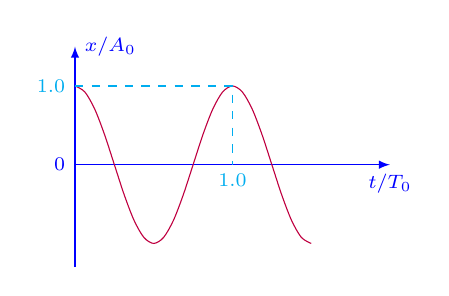
\begin{tikzpicture}[>=latex,font=\scriptsize]
    \draw[->,blue] (0,-1.3)--(0,1.5)node[right]{\(x\)/\(A_0\)};
    \draw[->,blue] (0,0)node[left]{0}--(4,0)node[below]{\(t\)/\(T_0\)};
    \draw[purple,domain=0:3,smooth] plot(\x,{cos(pi*\x r)});
    \draw[dashed,cyan] (0,1)node[left]{1.0}--(2,1)--(2,0)node[below]{1.0};
    \end{tikzpicture}
\item 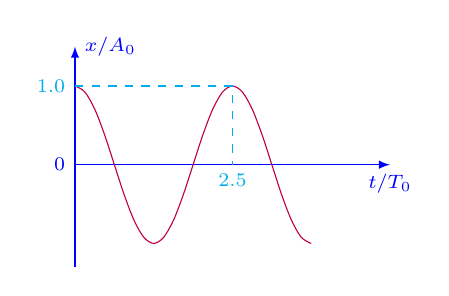
\begin{tikzpicture}[>=latex,font=\scriptsize]
    \draw[->,blue] (0,-1.3)--(0,1.5)node[right]{\(x\)/\(A_0\)};
    \draw[->,blue] (0,0)node[left]{0}--(4,0)node[below]{\(t\)/\(T_0\)};
    \draw[purple,domain=0:3,smooth] plot(\x,{cos(pi*\x r)});
    \draw[dashed,cyan] (0,1)node[left]{1.0}--(2,1)--(2,0)node[below]{2.5};
    \end{tikzpicture}
\item 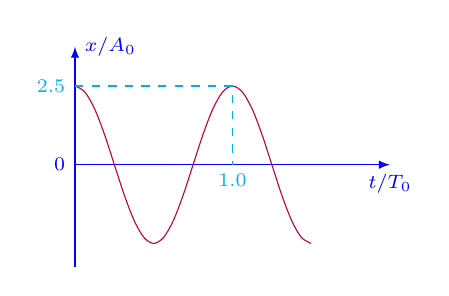
\begin{tikzpicture}[>=latex,font=\scriptsize]
    \draw[->,blue] (0,-1.3)--(0,1.5)node[right]{\(x\)/\(A_0\)};
    \draw[->,blue] (0,0)node[left]{0}--(4,0)node[below]{\(t\)/\(T_0\)};
    \draw[purple,domain=0:3,smooth] plot(\x,{cos(pi*\x r)});
    \draw[dashed,cyan] (0,1)node[left]{2.5}--(2,1)--(2,0)node[below]{1.0};
    \end{tikzpicture}
\item 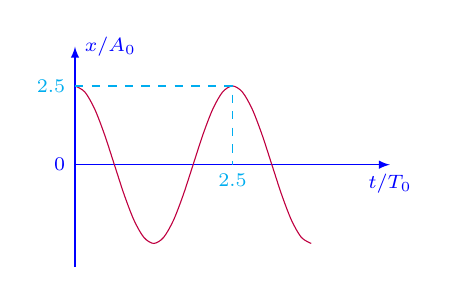
\begin{tikzpicture}[>=latex,font=\scriptsize]
    \draw[->,blue] (0,-1.3)--(0,1.5)node[right]{\(x\)/\(A_0\)};
    \draw[->,blue] (0,0)node[left]{0}--(4,0)node[below]{\(t\)/\(T_0\)};
    \draw[purple,domain=0:3,smooth] plot(\x,{cos(pi*\x r)});
    \draw[dashed,cyan] (0,1)node[left]{2.5}--(2,1)--(2,0)node[below]{2.5};
    \end{tikzpicture}
\end{choices}
\begin{answer}
    B\quad 提示：单摆周期公式\(T = 2\pi \sqrt{\frac{l}{g}}\)，月球重力加速度约为地球的\(\frac{1}{6}\)，\(\sqrt{6} = \sqrt{2}\cdot\sqrt{3} =2.45\)
\end{answer}